% Сборка из docs/report-stage2: xelatex report.tex
\documentclass[12pt,a4paper]{article}
\usepackage[margin=20mm]{geometry}
\usepackage{fontspec}
\setmainfont{Times New Roman}
\setmonofont{Menlo}[Scale=MatchLowercase]
\usepackage[russian]{babel}
\usepackage{graphicx}
\usepackage{pdflscape}
\usepackage{caption}
\usepackage{array,tabularx,booktabs}
\setlength{\parindent}{1.25cm}
\captionsetup{labelsep=endash}
\newcommand{\code}[1]{\texttt{\detokenize{#1}}}

\begin{document}

% Титульный лист
\begin{titlepage}
\begin{center}
    \LARGE Национальный исследовательский университет ИТМО\\[8mm]
    Факультет Программной Инженерии и Компьютерной техники\\[37mm]

    \huge \textbf{Информационные системы}\\[2mm]
    \textbf{Курсовая работа «РемКомСтрой»}\\[2mm]
    \Large Этап 2. Проектирование и реализация базы данных
\end{center}

\vfill

\begin{flushright}
    \large Выполнили:

    Кузьмин Дмитрий Анатольевич\\
    Калакин Яровлав Евгеньевич\\[3mm]

    Группа:

    P3309\\[3mm]

    Преподаватель:

    Николаев Владимир Вячеславович
\end{flushright}

\vfill

\begin{center}
    Санкт-Петербург 2026
\end{center}
\end{titlepage}

\begin{landscape}
\section{ER-модель}

\begin{center}
    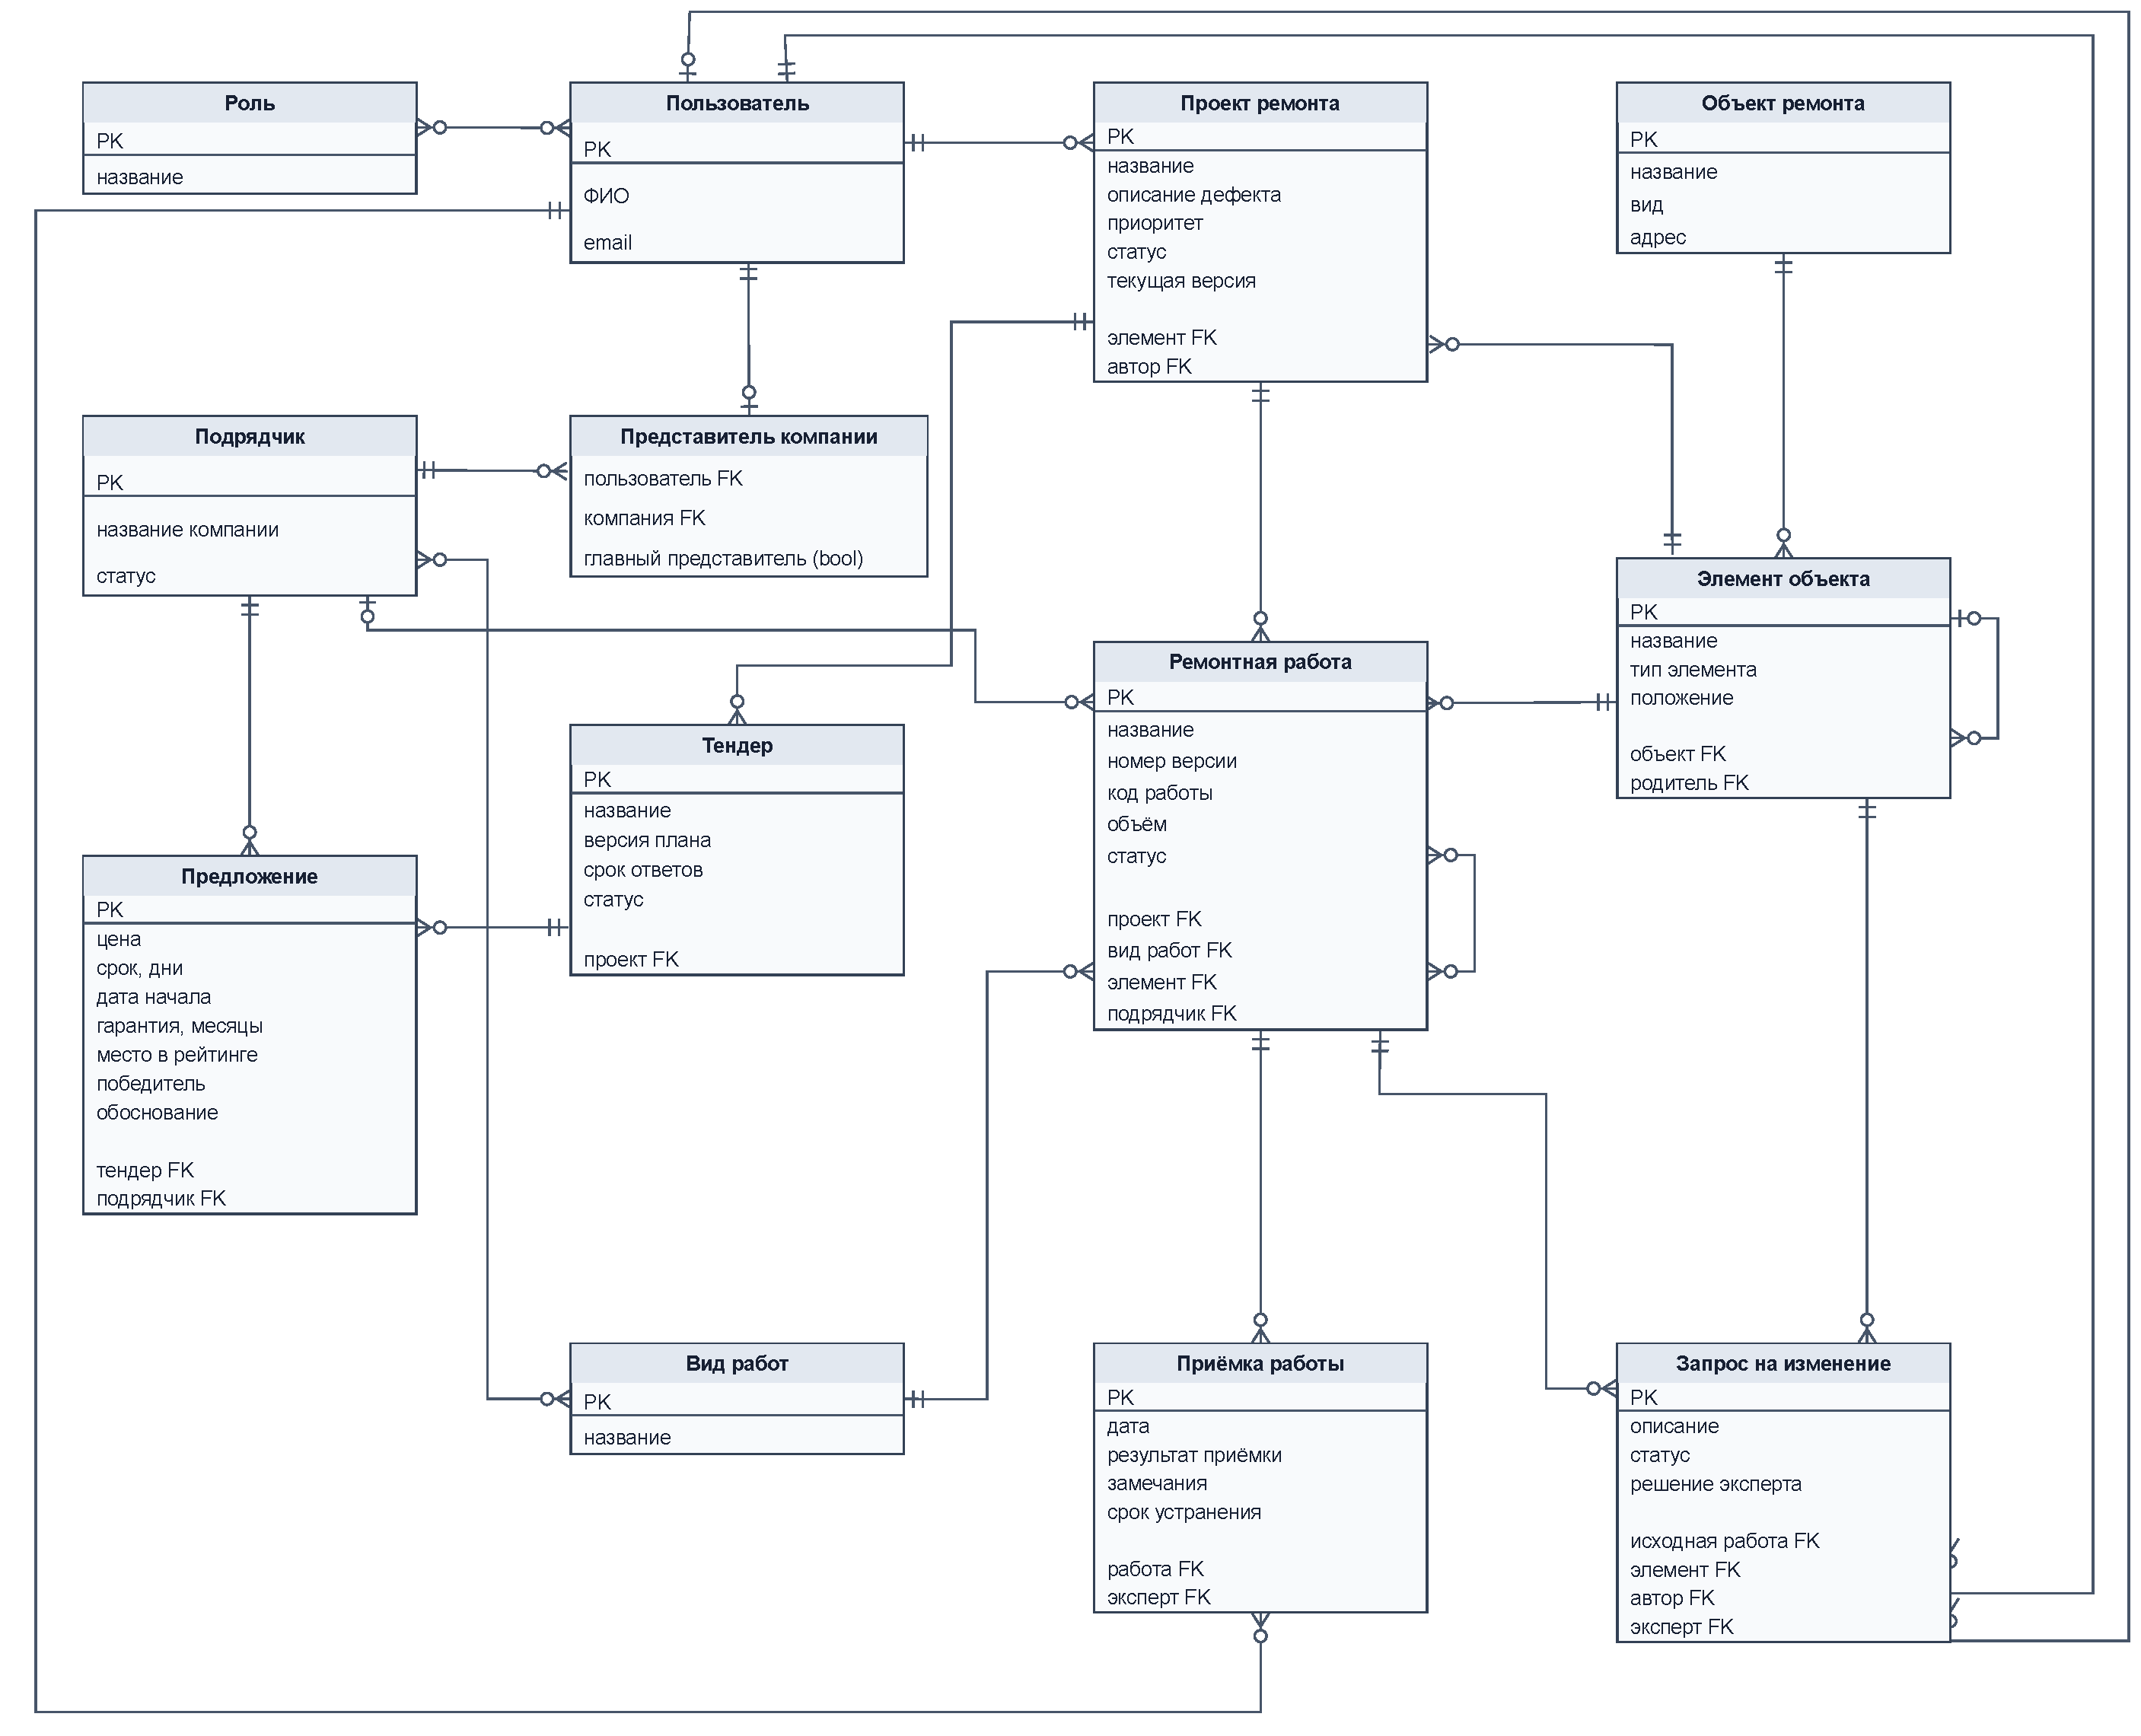
\includegraphics[width=\linewidth,height=.83\textheight,keepaspectratio]{er-diagram.pdf}
    \captionof{figure}{ER-диаграмма системы «РемКомСтрой»}
\end{center}
\clearpage

\section{Даталогическая модель}

\begin{center}
    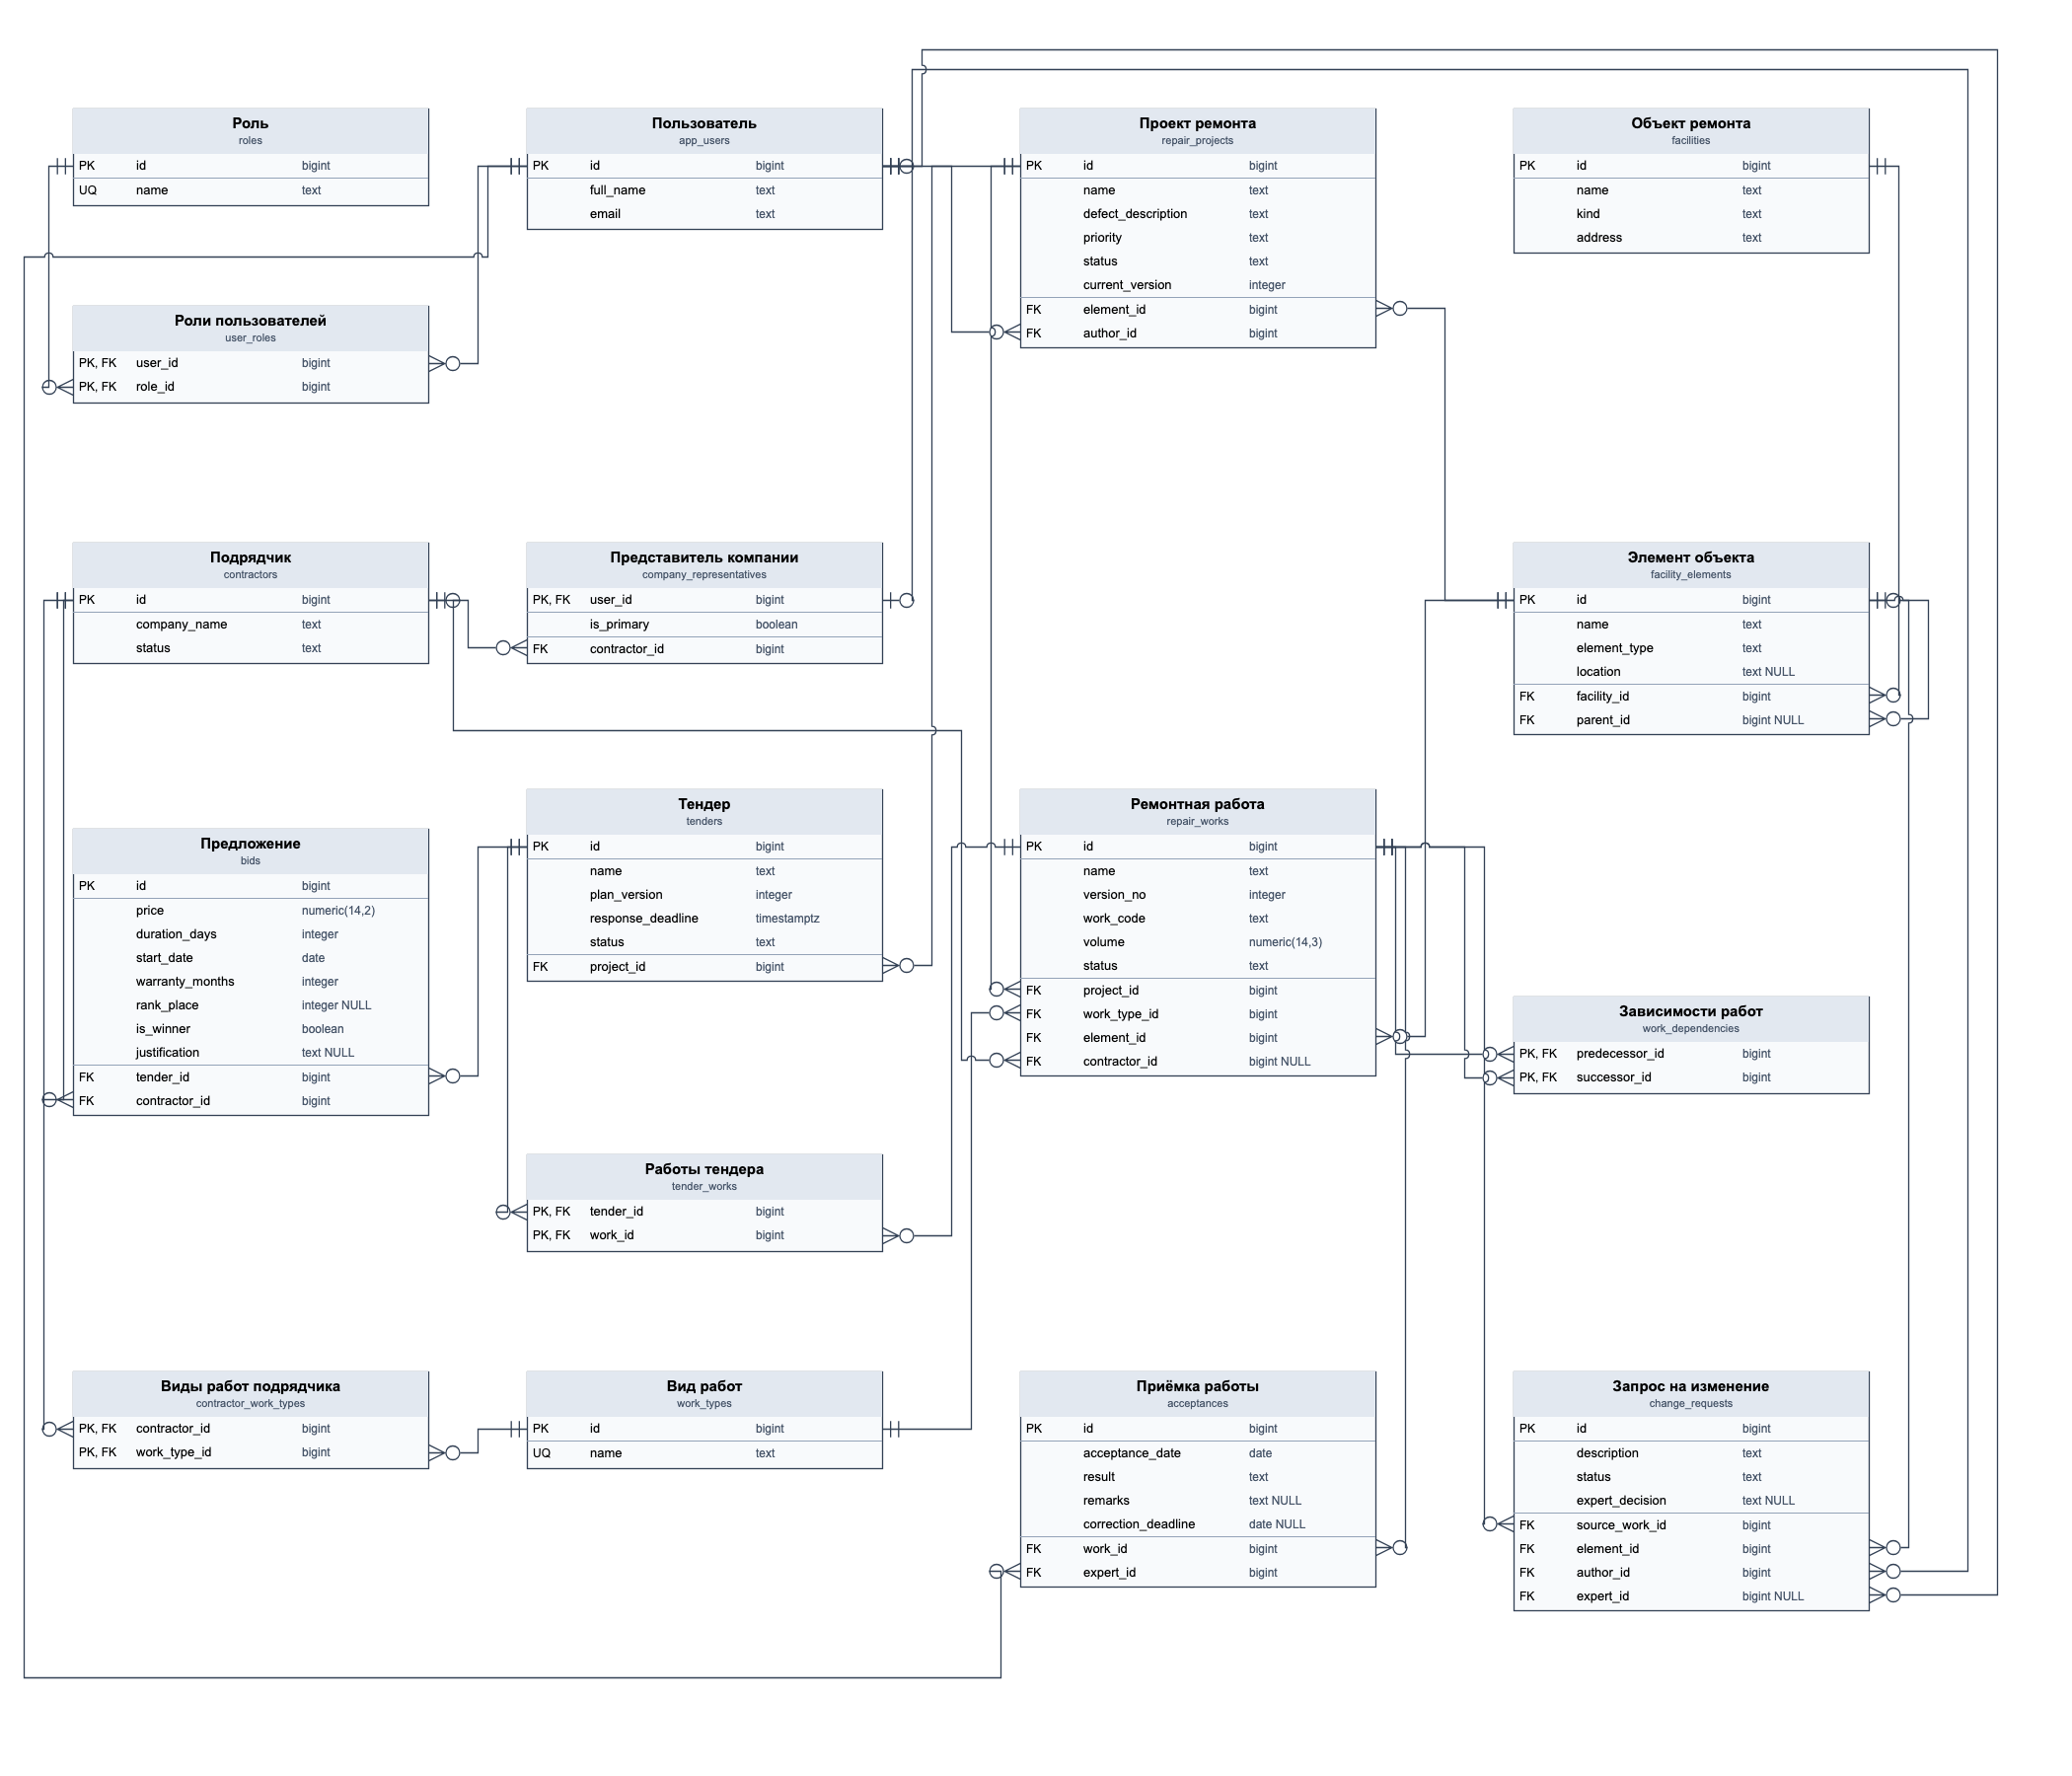
\includegraphics[width=\linewidth,height=.83\textheight,keepaspectratio]{../er/remkomstroy_logical.png}
    \captionof{figure}{Даталогическая модель базы данных}
\end{center}
\end{landscape}

\section{Реализация и целостность данных}

В PostgreSQL реализованы 17 таблиц. Для их размещения используется схема \code{s466402} базы \code{studs} на сервере Helios. В схеме имена таблиц курсовой начинаются с \code{c_}.

В таблицах заданы первичные и внешние ключи. Обязательные поля имеют ограничение \code{NOT NULL}. Проверки \code{CHECK} запрещают пустые названия и названия из одних пробелов, требуют положительную цену предложения и версию проекта не ниже единицы. При удалении записей каскадно удаляются связанные с ними строки из таблиц связей.

Реализованы два триггера.

\begin{description}
    \item[\code{change_request_done}] При переходе заявки в \code{DONE} версия проекта увеличивается на единицу. Функция \code{increment_project_version()} находит проект по исходной работе.
    \item[\code{facility_element_no_cycle}] При добавлении элемента с родителем или изменении его идентификатора либо родителя функция \code{prevent_element_cycle()} проверяет цепочку предков. Если в цепочке встречается сам элемент, операция отклоняется.
\end{description}

\section{Функции и процедура PL/pgSQL}

\begin{description}
    \item[\code{ready_repair_works}] Возвращает работы указанного проекта, назначенные подрядчику и ещё не начатые (\code{ASSIGNED}). В список входят работы без предшественников и работы, у которых все предшественники приняты.
    \item[\code{tender_bids}] Возвращает предложения по указанному тендеру. Для каждого предложения выводятся подрядчик, цена, срок, дата начала и гарантия. Предложения отсортированы по цене, а при равной цене — по идентификатору.
    \item[\code{register_acceptance}] Сохраняет результат приёмки и переводит работу из \code{ON_ACCEPTANCE} в \code{ACCEPTED} или \code{REWORK}. При возврате на доработку указываются замечания и срок исправления. Каждая проверка сохраняется отдельной записью.
\end{description}

\clearpage
\section{Индексы и обоснование}

\begin{description}
    \item[\code{c_repair_works_ready_idx}] Частичный индекс по подрядчику и проекту. В него входят только работы со статусом \code{ASSIGNED}. Индекс позволяет отобрать работы подрядчика перед проверкой их зависимостей.
    \item[\code{c_bids_tender_price_idx}] Индекс по тендеру, цене и идентификатору предложения. Позволяет выбрать предложения одного тендера в порядке цены, а при равной цене — в порядке идентификатора.
    \item[\code{c_acceptances_work_date_idx}] Индекс по работе, дате приёмки и идентификатору записи. Дата и идентификатор указаны в порядке убывания. Индекс подходит для просмотра истории приёмок и поиска последней проверки.
\end{description}

\end{document}
